\chapter{Contexto Teórico}\label{SM}

El Modelo Estándar (SM) de física de partículas ha demostrado ser extraordinariamente exitoso a la hora de describir numerosos resultados experimentales y predecir una gran variedad de fenómenos. El mérito del modelo reside en la unificación de las fuerzas fuerte, débil y electromagnética en una única teoría cuántica de campos de gauge, explicando como las partículas fundamentales y tres de las cuatro fuerzas de la naturaleza se relacionan entre sí.
Toma su forma actual con los trabajos de Glashow \cite{Glashowr}, Weinberg\cite{Weinberg} y Salam \cite{Salam} quienes unifican a las fuerzas electromagnética y débil (evocando en cierta forma la unificación de la electricidad y el magnetismo en la teoría electromagnética de Maxwell) e incorporan el mecanismo de Higgs\cite{MecHiggs1}\cite{MecHiggs2} al modelo. El descubrimiento de una nueva partícula en el 2012 en los experimentos ATLAS\cite{HiggsAtlas} y CMS\cite{HiggsCMS} en el LHC-CERN compatible con un Higgs como el presentado en el SM termina de completar las predicciones del modelo.\\
\indent En este capítulo se describe brevemente el Modelo Estándar y se introduce el concepto de Jets en el marco de la física de colisionadores de hadrones. 

\section{El Modelo Estándar en Física de Partículas}

El modelo estándar es una teoría de campos de gauge invariante ante transformaciones de simetría $SU_C(3)\otimes\,SU(2)_{L}\otimes\,U_Y(1)$. En él, los campos de materia son representados por partículas puntuales de spin 1/2 llamadas fermiones (y sus antipartículas), que interactúan entre sí mediados por partículas de spin 1 llamadas bosones de gauge.  

El espectro de partículas elementales del SM se presenta en la figura  \ref{fig:zoo}. Los fermiones del SM se dividen en dos familias: los \emph{quarks}, que interactúan a través de las fuerzas electrodébil y fuerte; y los \emph{leptones} que interactúan sólamente a través de la fuerza electrodébil (entre ellos, los neutrinos sólo interactúan a través de la fuerza débil). A su vez, los fermiones se pueden clasificar en tres generaciones, compuestas de un doblete de quarks (uno ``tipo up'' y uno ``tipo down'') y un doblete de leptones (uno ``tipo electrón'' y un neutrino); las tres de características similares a excepción de sus masas, que incrementan al subir de generación. La primera generación es la responsable de la materia ordinaria, compuesta de los quarks más livianos y el electrón.

Con la excepción de la fuerza gravitatoria, el SM establece que las fuerzas fundamentales que rigen la naturaleza son el resultado del intercambio de bosones de gauge entre los fermiones. La fuerza fuerte, descripta por el grupo de simetría \emph{SU(3)} de color, es mediada por los gluones, ocho en total, que poseen carga de color (análoga a la carga eléctrica)(ver \ref{QCD}). La fuerza electromagnética es mediada por el fotón y la fuerza débil por los bosones \emph{Z} y\emph{W}, estos últimos masivos. Estas dos fuerzas se unifican en la teoría electrodébil descripta por el grupo de simetrías $SU(2)_L \times U_Y(1)$. La ruptura espontánea de esta simetría (hacia $U_{EM}(1)$) a través del mecanismo de Higgs da origen a las diferentes masas de los bosones de gauge Z y W y a un nuevo bosón escalar de spin 1, dejando al fotón sin masa. A su vez, todos los fermiones que se acoplan al nuevo bosón de Higgs adquieren masa mediante la incorporación de términos de Yukawa al lagrangiano\cite{Gaillard}\cite{Halzen}. 

A pesar de ser la teoría de partículas más exitosa al momento, el SM presenta graves falencias: no da cuenta de la interaccón gravitatoria, ni de la materia y energía oscura, ni de la gran asimetría materia-antimateria presente en el universo. En él, tampoco se explica que los neutrinos tengan masa, ni el por qué de la estructura en generaciones de los fermiones. Otro aspecto no idóneo de la teoría es que posee 19 parámetros libres que deben determinarse a partir de observaciones experimentales.
Una introducción más completa al Modelo Estándar puede encontrarse en la referencia \cite{Halzen}

\begin{figure}[H]
        \centering
        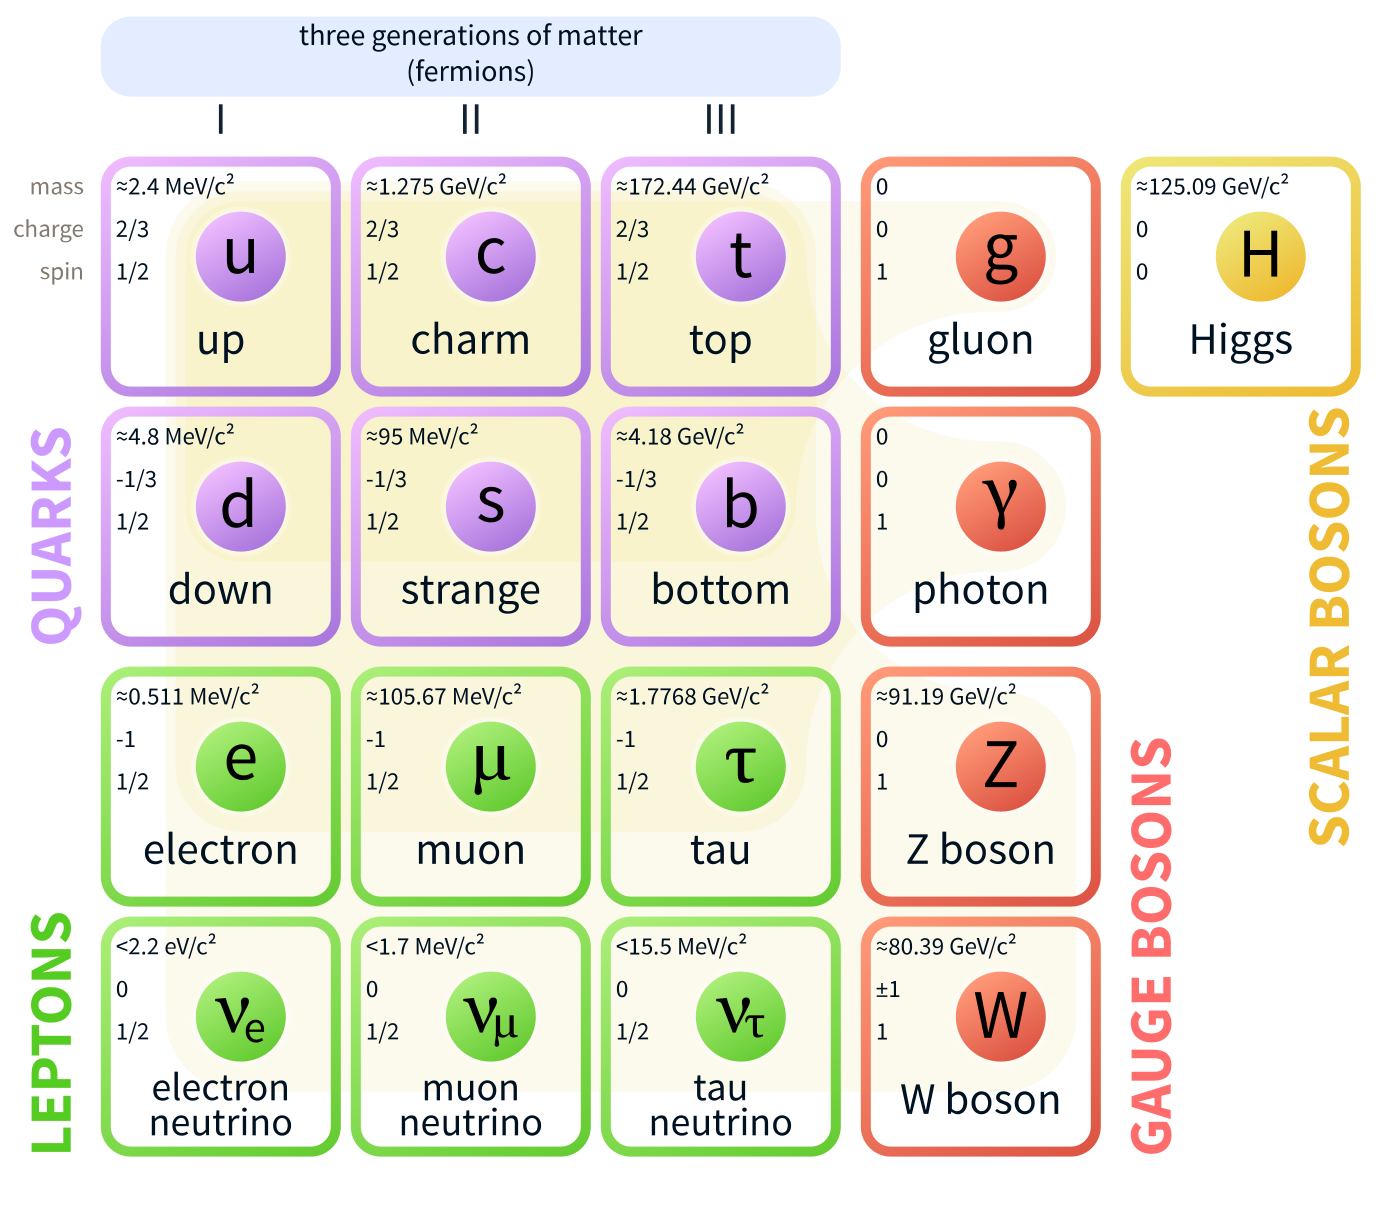
\includegraphics[width=0.7\linewidth]{images/zoo}
        \caption{Fermiones y Bosones del SM.}
        \label{fig:zoo}
\end{figure}

\section{Cromodinámica Cuántica}\label{QCD}
La cromodinámica cuántica (QCD), la componente $SU_c(3)$ del SM, describe la interacción fuerte entre quarks y gluones. Para que el color se conserve en las interacciones, los quarks deben portar un color (azul, rojo o verde), y los gluones un color y un anticolor.

\subsection{Dos propiedades de QCD}

 Al igual que en la electrodinámica cuántica o QED (teoría de campos de gauge que se refiere al electromagnetismo), el hecho de que el gluón no tenga masa da cuenta del rango infinito de la interacción fuerte; en cambio, en contraste con el fotón, como los gluones poseen carga de color, pueden acoplarse unos con otros. En consecuencia, la intensidad de la fuerza fuerte entre dos partículas con carga de color aumenta al aumentar la distancia entre ellas. Es por esto que los quarks y los gluones no pueden aparecer aislados sino que lo hacen en combinaciones incoloras llamadas hadrones. Se observan dos tipos de combinaciones con carga neta de color nula: los bariones, formados por tres quarks con diferentes colores o anticolores; y los mesones, parejas de quark-antiquark cuyos colores se cancelan\cite{Gaillard}.

La intensidad de la interacción entre partículas con carga de color está determinada por la constante de acoplamiento $\alpha_s$. En la figura \ref{fig:runningConstant} puede observarse el comportamiento de esta constante a diferentes escalas de energía $Q$ (transferencia de momento), observándose dos regímenes bien diferenciados. Por un lado, a baja escala de energía, es decir, para distancias grandes, la constante de acomplamiento aumenta, dando lugar al confinamiento mencionado.  Esto quiere decir que a medida que los quarks y gluones se separan aumenta la energía de ligadura entre ellos, y cuando esta se vuelve muy grande, se generan nuevos quarks y gluones con los que se combinan para formar hadrones. Este proceso se llama \emph{hadronización} y es un proceso no perturbativo. 

En cambio, para procesos que involucran grandes transferencias de momento, es decir $Q$ grande y distancias pequeñas, se observa que $\alpha_s$ se vuelve pequeña, y por lo tanto los quarks y los gluones pueden ser tratados como partículas libres (comportamiento conocido como \emph{libertad asintótica}). Estas dos características de QCD determinan que para procesos a alta escala de energías es posible usar la teoría de perturbaciones para realizar predicciones, pero no es posible hacerlo para procesos menos energéticos.
\begin{figure}[h]
    \centering
    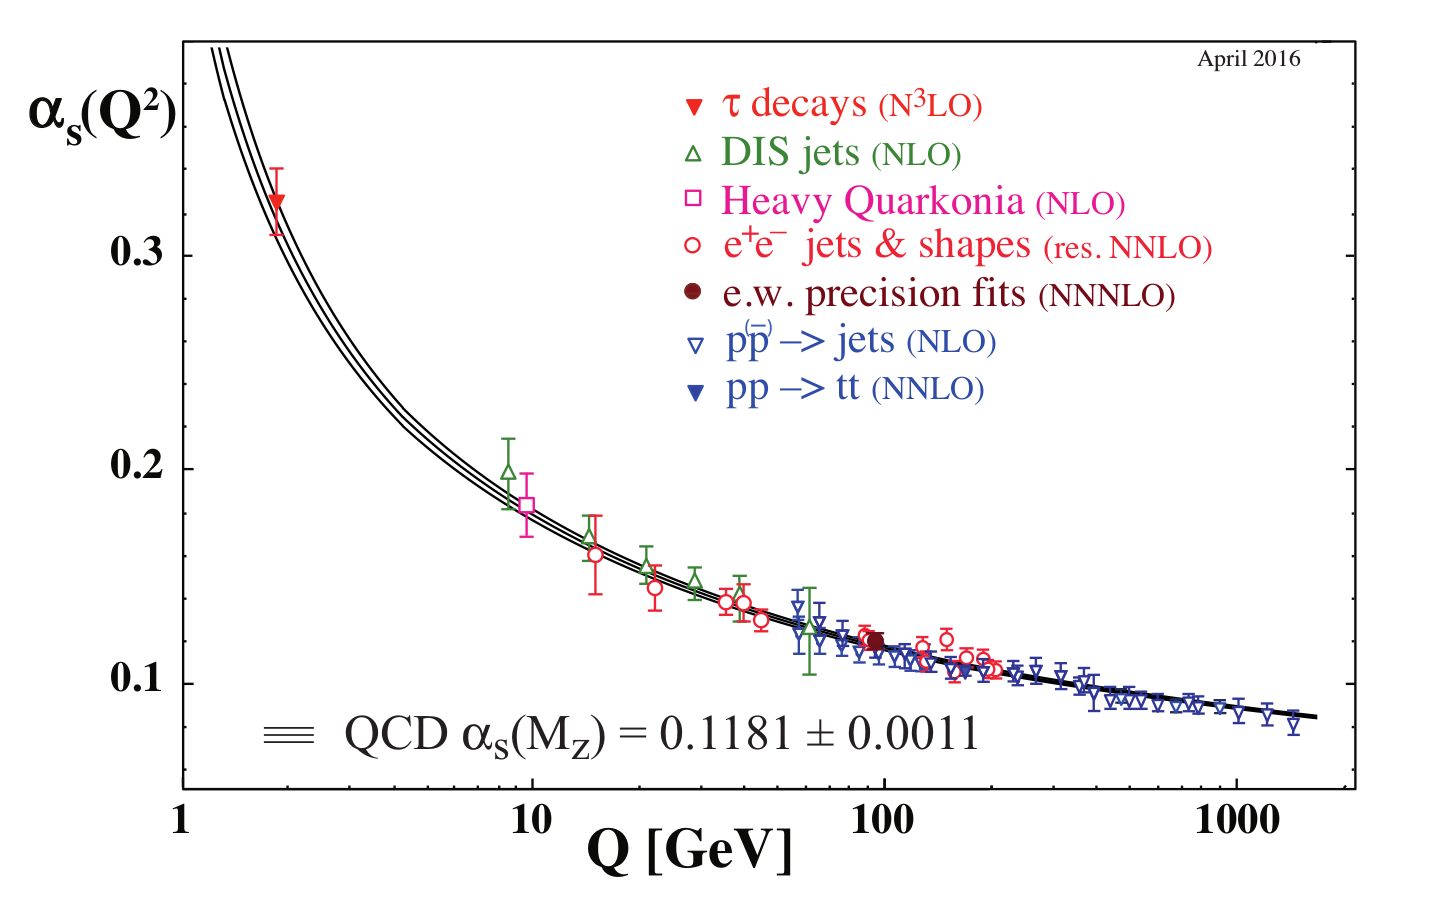
\includegraphics[width =0.8\linewidth]{images/runningConstant}
    \caption{Mediciones de $\alpha_s$ en diferentes experimentos en función de la escala de energía $Q$\cite{ParticleDataGroup}.}
    \label{fig:runningConstant}
\end{figure}

\section{Física de Colisionadores de Hadrones}

Los colisionadores de hadrones son las máquinas que proveen de la energía de centro de masa más alta disponible, permitiendo estudiar la estructura de la materia a las distancias más pequeñas en la búsqueda de nuevos fenómenos que permitan ir más allá del SM. Los hadrones, como por ejemplo el protón, son estados ligados incoloros de quarks y gluones, en su conjunto llamados partones. A continuación se presentan algunas de las consideraciones necesarias a tener en cuenta al estudiar procesos de scattering inelástico con hadrones en el estado inicial que permitan relacionar la teoría con lo observado en colisionadores.  

\subsection{Haciendo Predicciones de QCD}\label{predictions}

El modelo de partones interpreta a los constituyentes del hadrón como partículas cuasi-libres puntuales, de manera tal que se puede escribir a la sección eficaz de un proceso de scattering de hadrones con otra partícula a alta energía como una suma incoherente de secciones eficaces de los partones puntuales (del hadrón) con otra partícula. Los factores hadrónicos en la sección eficaz se parametrizan a través de ``funciones de estructura'', que no son calculables a partir de métodos perturbativos de QCD. El modelo, a su vez, expresa estas funciones en términos de funciones de distribución de partones (PDFs), que dan la distribución de momento longitudinal de los partones en un dado hadrón. Las PDFs se determinan a partir de datos experimentales en un dado proceso y luego se usan en la descripción de otros\cite{Greenberg}\cite{Bjorken}. Se considera entonces el \emph{hard scattering} (proceso dominante): un dado partón de un hadrón interactúa con un partón del otro hadrón. Esta interacción puede calcularse a través de cálculos perturbativos de QCD y es la que determina la escala de energía ($Q^2$) de la interacción fuerte. De esta manera, la sección eficaz para una colisión protón-protón se puede escribir como 

$$ \sigma_{p_1p_2\rightarrow X} = \sum_{i,j} \int dx_1 dx_2 \,f_{i/p_1}(x_1,\mu^2_F) f_{j/p_2}(x_2,\mu^2_F)\,\hat{\sigma}_{ij\rightarrow X}(x_1 x_2 s,\alpha_s(\mu^2_R),\mu^2_F,\mu^2_R)$$

\noindent donde $s$ es la energía de centro de masa de la colisión al cuadrado, $f_{i/p_1}(x_1,\mu^2_F)$ es la PDF correspondiente al partón de tipo $i$, en el protón $p_1$ que porta una fracción $x_1$ del momento de $p_1$, y $\mu_F$ es la escala de factorización\footnote{Escala que separa la física perturbativa de la no perturbativa.}. La sección eficaz para el proceso partónico, $\hat{\sigma}_{ij\rightarrow X}$ se puede calcular explícitamente usando teoría de perturbaciones a orden fijo, introduciendo una dependencia con la escala de renormalización\footnote{Escala para la cual las divergencias naturales de la sección eficaz son canceladas con contra-términos en el lagrangiano}, $\mu^2_R$. Así, la sección eficaz total de producción de $X$ se obtiene de sumar sobre todos los posibles sabores e integrando en todas las posibles fracciones de impulso.

Las partículas producto del hard scattering, sin embargo, no son las que se miden: mientras que los cálculos perturbativos de QCD involucran solamente partones, los estados finales de QCD consisten de hadrones, y, por lo tanto, la sección eficaz debe considerar todos los posibles estados hadrónicos finales. Físicamente, un partón energético se fragmenta (por ``showering'') en otros partones: gracias a la propiedad de confinamiento de QCD, se vuelve energéticamente favorable la creación de un par quark-antiquark del vacío, quienes en una escala de tiempo posterior se re-combinarán para formar hadrones (\emph{hadronización}). Como el partón original (proveniente del hard scatter) tenía momento, los hadrones resultantes se presentan como una lluvia de partículas colimadas en la misma dirección que el partón inicial, en lo que se llama un \emph{jet}. Como la transición partón-hadrón es no perturbativa, no es posible calcular en serie de perturbaciones una cantidad como puede ser el espectro de energía de hadrones específicos. Sin embargo, se pueden factorizar las contribuciones perturbativas y no perturbativas a través de funciones de fragmentación, análogas a las PDFs usadas para los hadrones del estado inicial y también determinadas vía resultados experimentales\cite{ParticleDataGroup}. Los hadrones resultantes usualmente son inestables y decaen en otras partículas con vida media lo suficientemente larga como para ser detectados. 

En una colisión \emph{pp}, además del \emph{hard scattering} y los decaimientos de sus productos, deben considerarse otros procesos a la hora de realizar predicciones que puedan compararse con los datos provistos por colisionadores. Uno de ellos es la radiación del estado inicial o \emph{ISR}: los partones incidentes en la colisión pueden radiar gluones y fotones vía radiación de Bremsstrahlung; y su análogo , la radiación de estado final, para partones producto de la interacción fuerte (FSR). Por otro lado, los otros quarks y gluones en los protones (que no conforman el \emph{hard scattering}) también pueden interactuar. Estas interacciones llamadas ``Multiple Parton Interactions''(MPIs) también tienen asociadas ISR y FSR.
Los quarks y gluones involucrados en el hard scattering y los MPIs toman una fracción de la energía total de los protones iniciales. La energía restante es llevada por los remanentes del haz de protones, este remanente junto con los MPIs conforman el ``evento subyacente''(UE).


Entonces, además del cálculo de la sección eficaz del hard scatter, es importante poder modelar los efectos no perturbativos (presentes en las PDFs, ISR, FSR, el evento subyacente y la hadronización) para poder realizar predicciones de eventos de QCD que puedan ser contrastadas con datos de colisiones. De esta manera, a través de generadores de Monte Carlo (MC) se puede tener acceso a eventos a nivel hadrónico, herramienta fundamental para todos los análisis que requieran estudiar la respuesta del detector a eventos de QCD.
\begin{figure}[h]
    \centering
    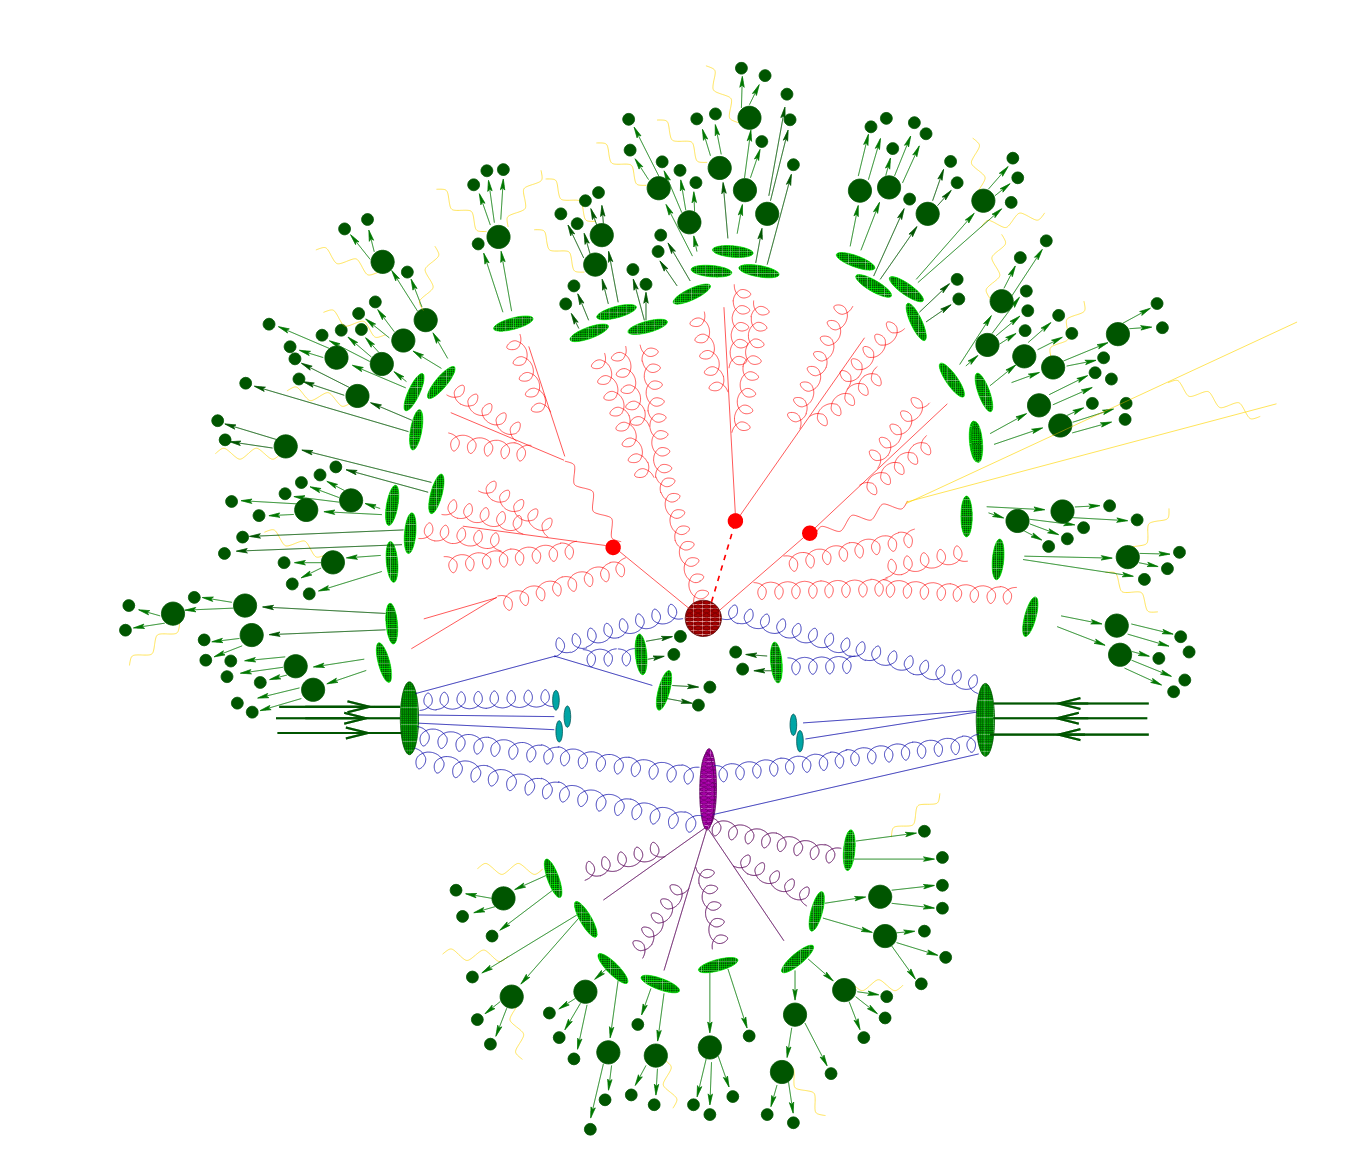
\includegraphics[width =0.8\linewidth]{images/MCgeneration}
    \caption{Simulación de Monte Carlo de una colisión. El hard scattering se muestra con un círculo rojo grande, los productos se muestran en círculos rojos más pequeños, y la lluvia partónica (QCD) en líneas rojas. A su vez, los partones que no conforman el evento principal pueden interactuar (círculo violeta), y los productos de esta interacción secundaria (UE) también pueden desencadenar una lluvia partónica. Los partones finales luego hadronizan (círculos en verde más claro), y estos hadrones finalmente  decaen en partículas más estables (círculos verde oscuro). En amarillo se indican procesos de Bremsstrahlung de QED, que pueden ocurrir en cualquier parte del proceso\cite{Sherpa}. }
    \label{fig:MCgeneration}
\end{figure}

La simulación de un evento a través de un generador de MC se esquematiza en la figura \ref{fig:MCgeneration}. Primero el hard scattering se simula a través de generadores de elementos de matriz que tienen en cuenta las PDFs. El siguiente paso es incorporar las lluvias de partones o ``parton showering'', usualmente basadas en la generación sucesiva y aleatoria de emisiones de gluones o decaimientos de ellos en pares quark-antiquark, cada una generada a una escala de energías inferior a la anterior. La lluvia de partones se detiene en una escala del orden de $1 GeV$, a partir de la cual se utiliza un modelo de hadronización para convertir a los partones resultantes en hadrones. Dos de los modelos más usados para simular la hadronización son el modelo de Lund \cite{Lund} y el de Clustering \cite{Cluster} . En el primero, la fuerza fuerte entre partones se modela como una ``cuerda''  de color de manera que la energía potencial de la cuerda aumenta a medida que los partones se separan. Eventualmente la cuerda se rompe y se forman nuevos partones que se combinan formando hadrones. El segundo modelo rompe cada gluón en un par $q\bar{q}$ y luego reagrupa en clusters incoloros que dan lugar a los hadrones. Hasta este punto es lo que se considera el ``truth level'', es decir esta parte de la simulación se realiza sin tener en cuenta la respuesta del detector\cite{ParticleDataGroup}. El siguiente paso involucra la reconstrucción de los eventos tal como serían observados experimentalmente a través de la simulación de la respuesta del detector a este input. 


\section{Interacción de las partículas con la materia}

En detectores como ATLAS en el LHC las partículas se detectan reconstruyendo su traza y midiendo su energía. En esta sección se introducen algunos de los principios físicos usados comúnmente en la detección de partículas. En este contexto, se introducen también los conceptos de calorimetría y lluvias de partículas; y un detalle de cómo se reconstruyen las trazas en ATLAS, y el lay-out del experimento se describen en el capítulo \ref{TheExperiment}.\\


La interacción de las partículas con la materia puede darse de diferentes maneras, entre ellas\cite{Instrumentation}:
\begin{itemize}

\item \emph{Ionización y excitación atómica}. Una partícula cargada que interactua con un átomo puede hacerlo vía la fuerza de Coulomb con los electrones atómicos.
Si la transferencia de energía es pequeña (una interacción distante) el electrón atómico pasará a un estado excitado; mientras que si la transferencia de energía es lo suficientemente grande para superar la energía de ligadura, el átomo se ionizará y el electrón atómico será liberado. Los fotones resultantes de la des-excitación (luz de centelleo) de los átomos y los electrones e iones producto de la ionización son capaces de generar señales medibles.
\item \emph{Scattering múltiple, bremsstrahlung y producción de pares}. La interacción Coulombiana de una partícula con los núcleos atómicos del material del detector produce una desviación de la trayectoria de la partícula, esto recibe el nombre de ``scattering múltiple''. Esta deflexión induce una aceleración, y, por lo tanto, la emisión de radiación electromagnética, efecto denominado Bremsstrahlung. Además, un fotón de alta energía tiene una probabilidad de producir un par electrón-positrón en la vecindad de los núcleos. La distancia media que viaja un fotón de alta energía en el material antes de convertirse en un par electrón-positrón está dada aproximadamente por la longitud de radiación $X_0$ (distancia recorrida para la cual la energía del electrón cayó a $1/e$ de la energía inicial). Estos dos procesos dados alternadamente resultan en una cascada electromagnética de cada vez más electrones y positrones de menor energía, hasta que se ``detienen'' en el material cuando su energía cae por debajo de una energía crítica a partir de la cual disipan su energía por ionización y excitación.
\item \emph{Radiación de transición}. La radiación de transición se emite cuando una partícula cargada atraviesa la interfaz entre dos materiales de diferente permitividad. La probabilidad de emisión es proporcional al factor de Lorentz $\gamma$ de la partícula, y sólo resulta apreciable para partículas ultra relativistas, con lo cual es útil para distinguir electrones de hadrones. 
\item \emph{Radiación Cerenkov}. Las partículas cargadas que atraviesan un material a velocidades mayores que la velocidad de la luz en dicho material producen una onda de choque electromagnética que se evidencia como radiación electromagnética en el rango visible y ultravioleta.
\end{itemize}

En ATLAS se aprovechan los primeros dos ítems en la determinación de la energía de las partículas en los llamados calorímetros, mientras que la reconstrucción de trazas se basa en los procesos de ionización y radiación de transición (ver sección \ref{layout}).

\subsection{Calorimetría}\label{Lluvias}

En física de partículas, un calorímetro es un tipo de detector que mide la energía de una partícula frenándola por completo y traduciendo esta energía en una señal eléctrica. Como consecuencia, la partícula ya no se encuentra disponible para más mediciones. Si la energía de la partícula se encuentra bien por encima del umbral de scattering inelástico entre dicha partícula y el material del detector, el proceso de pérdida de energía se da con una cascada de partículas de menor energía, en número acorde con la energía incidente. Las partículas cargadas en la lluvia eventualmente pierden su energía a través de procesos más elementales, principalmente, ionización y excitaciones a nivel atómico. La señal calorimétrica corresponde a la suma de estas pérdidas elementales. Sólo interacciones de naturaleza electromagnética o fuerte contribuyen a las señales calorimétricas, partículas que sólo pueden interactuar débilmente escapan de la detección calorimétrica. Se distinguen dos tipos de lluvias:\\


\indent \emph{Lluvias electromagnéticas.} Como ya se mencionó, el proceso de creación de pares (dominante para fotones con energía por encima de 1MeV) alternado con Bremsstrahlung (dominante para electrones y positrones por encima de una energía crítica $\approx 550 MeV/Z$) lleva a un electrón o fotón a producir una lluvia de electrones o positrones, con energías cada vez menores hasta que se detienen en el material debido a pérdida por ionización. La cantidad total de ionización producida da una medida de la energía de la partícula.\\
 
\indent \emph{Lluvias hadrónicas.} Existe el efecto análogo al bremsstrahlung electromagnético para interacciones  hadrónicas. Cuando un hadrón de alta energía interactúa con el material del detector, típicamente choca contra un núcleo atómico y produce la fragmentación del mismo y hadrones secundarios que luego pueden interactuar con otros núcleos o bien decaer en otros hadrones. La lluvia hadrónica continuará hasta que los hadrones no tengan suficiente energía para romper más núcleos. En este punto la pérdida de energía se dará principalmente por ionización o absorción en algún proceso nuclear\cite{DetectorBook6}. La escala de longitud en este caso es la longitud de interacción hadrónica ($\lambda$) y es significativamente mayor que la longitud de radiación $X_0$ mencionada para el caso electromagnético (por ejemplo, para el caso del hierro, es diez veces mayor). Esto quiere decir que las lluvias hadrónicas deben avanzar sobre más material que una lluvia EM para depositar toda su energía. Es por esto que los calorímetros hadrónicos suelen ser de materiales más densos y estar ubicados más allá de los EM \cite{Instrumentation}. En una lluvia hadrónica, la energía se transfiere al medio a través de interacciones electromagnéticas (ionización, $\pi^0 \rightarrow \gamma\gamma$, etc.) y hadrónicas (fisión, recombinación en hadrones, scattering elástico de neutrones, etc.). En la componente hadrónica, la energía utilizada en ligaduras nucleares, excitaciones nucleares, y en reducir la velocidad de los neutrones no puede ser detectada por el calorímetro. De la misma manera, la producción de neutrinos y muones que escapan del detector da por resultado energía que tampoco puede ser detectada. Por estos motivos, y considerando además que la composición de partículas en una lluvia hadrónica es de naturaleza estocástica, se tiene que la respuesta al medir energía depositada vía interacciones electromagnéticas es mayor que en el caso hadrónico. \\
 
 
En simulaciones de MC, para reproducir las señales calorimétricas medidas en ATLAS, los eventos generados a ``truth level'' son propagados a través de una simulación completa del detector basada en GEANT4 \cite{AtlasSimulation}. A esta altura, las simulaciones de MC y los datos recolectados del detector están en pie de igualdad, de modo que en ambos casos se pueden utilizar las mismas herramientas de reconstrucción de objetos.

